\documentclass{jknotes}
\usepackage{../joshkirklin}

\setmathfont{Latin Modern Math}
\setmathfont{GFS NeoHellenic Math}[range=bfsfup/{greek,Greek}->it]
\setmathfont{GFS NeoHellenic Math}[range=sfup/{latin,Latin}->it]

\usetikzlibrary{shapes.misc}
\renewcommand{\u}{\symbf{u}}

\tikzset{cross/.style={cross out, draw=black, minimum
size=2*(#1-\pgflinewidth), inner sep=0pt, outer sep=0pt}}
%default radius will be 1pt. 

\newcommand{\myol}[2][3]{{}\mkern#1mu\overline{\mkern-#1mu#2}}

\begin{document}

\institution{Cambridge Part III Maths}
\title{Hydrodynamic Stability}
\lecturer{Prof. Richard Kerswell}
\notetaker{Charles Powell}
\date{Lent 2020}

\maketitle
\suggestionsspiel
\tableofcontents

\section{Introduction}
We are typically interested in whether a given flow solution $\u(\x,t)$ is
`stable', certainly to small (infinitesimal) disturbances and perhaps to
larger perturbations too. We perturb $\u(\x)$ to $\u(\x) + \hat{\u}(\x,t)$ and
define the \emph{perturbation energy} as
\begin{equation}
	E(t) \equiv \int \frac{1}{2}\hat{\u}^2(\x,t) \, \diffd V
\end{equation}
A solution is said to be stable if
\begin{equation}
	\lim_{t \to \infty} \frac{E(t)}{E(0)} = 0
\end{equation}
for all perturbations $\hat{\u}$. Conversely, if there exists $\hat{\u}$ such
that $E(t) \not\rightarrow 0$ then $\u$ is unstable. The nature of $E(0)$
determines the type of perturbation:
\begin{itemize}
	\item If $E(0) \to 0$ we have an infinitesimal disturbance
	\item If $E(0) < \delta$ then we probe finite amplitude disturbances
	\item If $E(0) \to \infty$ this probes the \emph{global} stability
\end{itemize}

In the first 9 lectures we focus on the first situation, which is linear
stability analysis. Consider the Navier-Stokes equations
\begin{align}
	\frac{\partial \u}{\partial t} + \u \cdot \nabla \u + \nabla p =
	\frac{1}{\text{Re}} \nabla^2 \u
\end{align}

If $\symbf{U}(\x)$ is a steady (basic) solution then
\begin{equation}
	\symbf{U}\cdot\nabla\symbf{U} + \nabla P = \frac{1}{\text{Re}} \nabla^2
	\symbf{U}
\end{equation}
Let $\u = \symbf{U}(\x) + \hat{\u}(\x,t), p = P + \hat{p}$. Then
\begin{equation}
	\frac{\partial \hat{\u}}{\partial t} + \u \cdot \nabla \symbf{U} +
	\symbf{U} \cdot \nabla \hat{\u} + \cancel{\hat{\u}\cdot\nabla\hat{\u}} +
	\nabla \hat{p} = \frac{1}{\text{Re}} \nabla^2 \hat{\u}
\end{equation}
The term $\hat{u}\cdot\nabla \symbf{U}$ is stabilising whilst the term
$\nabla^2 \hat{u} / \text{Re}$ is stabilising. Therefore, we expect stability
as $\text{Re} \to 0$ as this term dominates, and instability as $\text{Re} \to
\infty$. Thus there exists some value $\text{Re}_{\text{crit}}$ at which
instability arises. We will ask what this value is, and what is the form of initial
instability/mode/pattern?

\section{Kelvin-Helmholtz instability}
See Drazen (2002), section 3.3, pages 47--50. Here we take a different approach
and derive Rayleigh's equation (example 8.3, page 151 of Drazen). 

\begin{center}
	\begin{tikzpicture}
		\draw[thick,->] (-3, 0) -- (3, 0) node[right] {$x$};
		\draw[dashed,->] (0, -1.5) -- (0, 1.5) node[above] {$z$};
		\draw[blue,dashed] (1.5, 0) -- (1.5, 1.4);
		\draw (1.5, 0) node[below] {$U$};
		\draw (-1.5, 0) node[above] {$U$};
		\draw[blue,dashed] (-1.5, 0) -- (-1.5, -1.4);

		\draw[blue,->] (0, 0.4) -- (1.5, 0.4);
		\draw[blue,->] (0, 0.8) -- (1.5, 0.8);
		\draw[blue,->] (0, 1.2) -- (1.5, 1.2);
		\draw[blue,->] (0, -0.4) -- (-1.5, -0.4);
		\draw[blue,->] (0, -0.8) -- (-1.5, -0.8);
		\draw[blue,->] (0, -1.2) -- (-1.5, -1.2);
	\end{tikzpicture}
\end{center}

Consider a flow $\u = U(z)\hat{\x}$ where
\begin{equation}
	U(z) = \begin{cases} U & z > 0 \\ -U & z < 0 \end{cases}
\end{equation}
The linearised, \emph{inviscid} equation for perturbation $\hat{\u}$ is
\begin{align}
	\frac{\partial \hat{\u}}{\partial t} + \hat{w}U'\hat{\x} + U
	\frac{\partial \hat{\u}}{\partial x} + \nabla \hat{p} &= 0 \\
	\nabla \cdot \hat{\u} &= 0 
\end{align}
The boundary conditions are $\hat{\u} \to 0$ as $z \to \pm \infty$, i.e. no
energy radiated in from infinity. We will work in 2D $(\hat{u},\hat{w}) =
(\psi_z, -\psi_x)$ and let $\psi(x,z,t) = \phi(z) e^{i\alpha(x-ct)}$ where $c$
is a complex eigenvalue, currently unknown. Formally, this is equivalent to
taking a Fourier transform. We have
\begin{equation}
	i\alpha (U-c) \begin{pmatrix} \phi' \\ -i\alpha \phi \end{pmatrix} +
	\begin{pmatrix} -i\alpha U' \phi \\ 0 \end{pmatrix} + \begin{pmatrix} i
\alpha p \\ \frac{\partial p}{\partial z} \end{pmatrix} = 0
\end{equation}
We can eliminate $p$ via $\partial_z (\text{top}) - i\alpha(\text{bottom})$ to
get
\begin{equation}
	(U-c)(\phi''-\alpha^2 \phi) - U'' \phi = 0
\end{equation}
with boundary conditions $\phi \to 0$ as $z \to \pm \infty$. This is
\emph{Rayleigh's equation}. Note that $c$ is the crucal eigenvalue. We wish to
know when $c_i = \Im(c) > 0$ as a function of $U(z)$, as $c_i$ is the growth
rate:
\begin{equation}
	\hat{u} \propto e^{i\alpha(x-ct)} = e^{i\alpha(c-c_r t - i c_i t)} =
		e^{i\alpha(x-c_r t) + \alpha c_i t}
\end{equation}
Note the following:
\begin{itemize}
	\item There is a symmetry $\alpha \mapsto -\alpha$, so without loss of
		generality we consider $\alpha > 0$.
	\item The complex conjugate is also a solution with $c \mapsto c^*$. Hence
		an unstable mode has a damped partner, so we have stability only if
		all modes are `neutral' i.e. $c_i = 0$. 
	\item There is a possible singularity at $y$ where $U(y) = c$, called the
		\emph{critical layer}. If $c$ is real, see later.
\end{itemize}

We now solve Rayleigh's equation with $U(z)$ defined as before. We solve above
and below $z=0$ and piece the solutions together. Since $U'' = 0$, we have
\begin{equation}
	\phi'' = \alpha^2 \phi
\end{equation}
which admits a solution satisfying the boundary conditions:
\begin{equation}
	\phi = \begin{cases} A^{-\alpha z} & z > 0 \\ B e^{\alpha z} & z < 0 
	\end{cases}
\end{equation}

The matching conditions at $z=0$ are
\begin{enumerate}
	\item Pressure $\hat{p}$ continuous at $z=0$, with $\hat{p}$ given by:
		\begin{equation}
			\hat{p} = U' \phi - (U-c) \phi'
		\end{equation}
	\item Kinematic condition at the surface:
		\begin{equation}
			\frac{\diffD}{\diffD t} \left( z - \zeta(x,t)\right) = 0
		\end{equation}
		where $z=\zeta(x,t)$ is the position of the surface.
		After linearising, we have
		\begin{equation}
			 w - \frac{\partial \zeta}{\partial t} - U\frac{\partial
			 \zeta}{\partial x} = 0
		\end{equation}
	 	Inserting the form of $w$ and $U$ we require that
	 	\begin{equation}
		 	\zeta = - \frac{\phi}{U-c}
	 	\end{equation}
	 	is continuous across $z=0$.
\end{enumerate}
Requiring $p$ continuous gives
\begin{equation}
	-(U-c)A(-\alpha) = - (-U-c)B(\alpha)
\end{equation}
Requiring $\zeta$ continuous gives
\begin{equation}
	\frac{A}{U-c} = \frac{B}{-U-c}
\end{equation}
Hence we have
\begin{equation}
	(U-c)^2 = -(U+c)^2
\end{equation}
i.e. $c = \pm i U$ so the growth rate is $\alpha U$. Thus the flow is unstable
to waves of all wavelengths. The instability may be remedied 
\begin{itemize}
	\item by adding a density stratification, which stabilises long
		wavelengths (small $\alpha$)
	\item by adding surface tension, which stabilises short wavelengths (large
		$\alpha$), e.g. Drazen page 50 equation 3.21.
\end{itemize}

\section{Thermal instabilities: convection}
Consider two parallel plates separated by distance $L$ with fluid subject to
gravity and temperatue difference $\Delta T$ between the plates. The lower
plate is heated. 
\begin{center}
	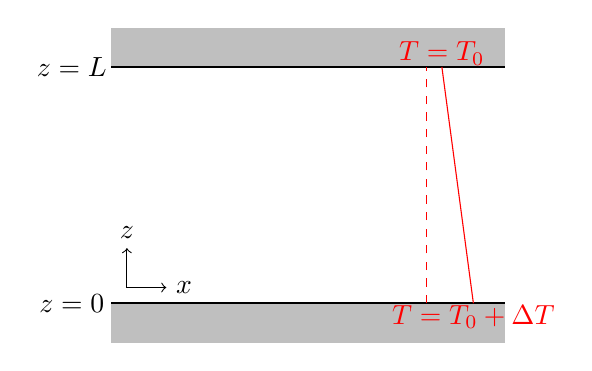
\begin{tikzpicture}
		\draw[draw=none,fill=gray!50] (0,0) rectangle (5,-0.5);
		\draw[thick] (0,0) -- (5, 0);
		\draw[draw=none,fill=gray!50] (0,3) rectangle (5,3.5);
		\draw[thick] (0,3) -- (5, 3);

		\draw[->] (0.2, 0.2) -- (0.7, 0.2) node[right] {$x$};
		\draw[->] (0.2, 0.2) -- (0.2, 0.7) node[above] {$z$};
		\draw (-0.5, 0) node {$z=0$};
		\draw (-0.5, 3) node {$z=L$};
		\draw[red,dashed] (4, 0) -- (4, 3);
		\draw[red] (4.2, 3) -- (4.6, 0);
		\draw[red] (4.2, 2.9) node[above] {$T=T_0$};
		\draw[red] (4.6, 0.1) node[below] {$T=T_0+\Delta T$};
	\end{tikzpicture}
\end{center}

The basic state consists of no motion, with heat transfer by conduction only.
\paragraph{Governing equations.}
The governing equations are 
\begin{align}
	\rho \frac{\diffD \u}{\diffD t} + \nabla p &= \mu \nabla^2 \u + \rho g
	\hat{\symbf{z}} \\
	\frac{\partial T}{\partial t} + \u \cdot \nabla T &= \kappa \nabla^2 T \\
	\frac{\diffD \rho}{\diffD t} + \rho \nabla \cdot \u &= 0
\end{align}
We need a relationship between $\rho$ and $T$. Most cases of interest have
$\Delta T$ and $\Delta \rho$ small, i.e. $\Delta \rho \ll \rho_0, \Delta T \ll
T_0$. Two consequences of this assumption are:
\begin{enumerate}
	\item We can Taylor expand $\rho = \rho(T)$:
		\begin{equation}
			\rho \approx \rho(T_0) \left[ 1 - \alpha(T-T_0)\right]
		\end{equation}
		where $\alpha > 0$ is the coefficient of thermal expansion, such that
		$T$ increases when $\rho$ decreases. We write $\rho_0 = \rho(T_0)$.
	\item We can adopt a Boussinesq approximation: acknowledge density changes
		only in the buoyancy term $\rho g \hat{\symbf{z}}$. Importantly, we
		can assume the fluid is incompressible.
\end{enumerate}

Define $\theta = T - T_0$. The governing equations are now
\begin{align}
	\rho_0 \frac{\diffD \u}{\diffD t} + \nabla p &= \mu \nabla^2 \u +
	\rho_0(1-\alpha \theta)g \hat{\symbf{z}} \\
	\frac{\partial \theta}{\partial t} + \u \cdot \nabla \theta &= \kappa
	\nabla^2 \theta \\
	\nabla \cdot \u &= 0
\end{align}

The basic state is $u = 0, \theta = \Delta T (1-z/L)$ and
\begin{equation}
	\frac{\diffd p}{\diffd z} = -\rho_0 (1-\alpha \Delta T(1-z/L))g
\end{equation}

We now non-dimensionalise using scalings $t \sim L^2/\kappa, u \sim \kappa/L,
\theta \sim \Delta T$, e.g. $\theta = \Delta T \theta^*$ where $\theta^*$ is
the non-dimensionalised variable. We normalise the $\frac{\diffD \u^*}{\diffD
t^*}$ term, to get:
\begin{align}
	\frac{\diffD \u^*}{\diffD t^*} + \nabla^* p^* &= \frac{\mu}{\rho_0 \kappa}
	\nabla^{*2} \u^* + \frac{\alpha g \Delta T L^3}{\kappa^2} \theta^* \hat{\symbf{z}} \\
	\frac{\partial \theta^*}{\partial t^*} + \u^* \cdot \nabla^* \theta^* &=
	\nabla^{*2} \theta^* \\
\end{align}
Define the \emph{Prandtl number} 
\begin{equation}
	\sigma \equiv \frac{\nu}{\kappa} = \frac{\mu}{\rho_0 \kappa}
\end{equation}
which is the ratio of viscous/momentum to thermal diffusivity. Typical values
are $0.72$ in air, $7$ in water, $10^5$ in magma. We also define the
\emph{Rayleigh number}
\begin{equation}
	\text{Ra} \equiv \frac{\alpha \Delta T g L^3}{\kappa \nu}
\end{equation}
which is the ratio of destabilising buoyancy to stabilising diffusion.
Dropping the $^*$ notation, we have
\begin{align}
	\frac{\partial \u}{\partial t} + \u \cdot \nabla \u + \nabla p &= \sigma
	\nabla^2 \u + \sigma \text{Ra} \theta \hat{\symbf{z}} \\
	\frac{\partial \theta}{\partial t} + \u \cdot \nabla \theta &= \nabla^2
	\theta \\
	\nabla \cdot \u &= 0
\end{align}

\paragraph{Boundary conditions.}
There are three combinations of boundary condition available in this problem.
\begin{center}
	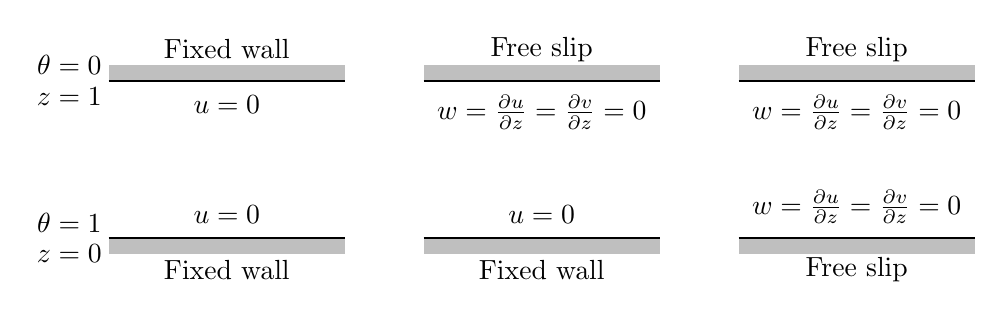
\begin{tikzpicture}
		\draw (-0.5, 0.2) node {$\theta = 1$};
		\draw (-0.5, -0.2) node {$z = 0$};
		\draw (-0.5, 2.2) node {$\theta = 0$};
		\draw (-0.5, 1.8) node {$z = 1$};

		\draw[fill=gray!50,draw=none] (0,0) rectangle (3,-0.2);
		\draw[fill=gray!50,draw=none] (0,2) rectangle (3,2.2);
		\draw[thick] (0,0) -- (3, 0);
		\draw[thick] (0,2) -- (3, 2);

		\draw (1.5, 0.3) node {$\u = 0$};
		\draw (1.5, 1.7) node {$\u = 0$};

		\draw (1.5, -0.4) node {Fixed wall};
		\draw (1.5, 2.4) node {Fixed wall};

		\begin{scope}[shift={(4, 0)}]
			\draw[fill=gray!50,draw=none] (0,0) rectangle (3,-0.2);
			\draw[fill=gray!50,draw=none] (0,2) rectangle (3,2.2);
			\draw[thick] (0,0) -- (3, 0);
			\draw[thick] (0,2) -- (3, 2);

			\draw (1.5, 0.3) node {$\u = 0$};
			\draw (1.5, 1.6) node {$w = \frac{\partial u}{\partial z} =
			\frac{\partial v}{\partial z} = 0$};

			\draw (1.5, -0.4) node {Fixed wall};
			\draw (1.5, 2.4) node {Free slip};
		\end{scope}
		\begin{scope}[shift={(8, 0)}]
			\draw[fill=gray!50,draw=none] (0,0) rectangle (3,-0.2);
			\draw[fill=gray!50,draw=none] (0,2) rectangle (3,2.2);
			\draw[thick] (0,0) -- (3, 0);
			\draw[thick] (0,2) -- (3, 2);

			\draw (1.5, 1.6) node {$w = \frac{\partial u}{\partial z} =
			\frac{\partial v}{\partial z} = 0$};
			\draw (1.5, 0.4) node {$w = \frac{\partial u}{\partial z} =
			\frac{\partial v}{\partial z} = 0$};

			\draw (1.5, -0.4) node {Free slip};
			\draw (1.5, 2.4) node {Free slip};
		\end{scope}
	\end{tikzpicture}
\end{center}

The double fixed wall case is easiest to replicate in a lab, whilst the double
free slip case is the easiest analytically, which we shall use.

\paragraph{Basic state.}
In the basic state we have conductive profile $\u_0 = 0, \theta_0 = 1-z$ and
from integration $p_0 = \sigma \text{Ra}( z - \frac{1}{2}z^2)$. We generate
linearised equations for perturbations $\theta = \theta_0 + \theta', \u = \u_0
+ \u', p = p_0 + p'$. As usual with linear stability analysis, we assume
$(\theta, \u', p')$ are small.

\begin{align}
	\frac{\partial \u'}{\partial t} + \cancel{\u' \cdot \nabla \u'} + \nabla
	p' &= \sigma \nabla^2 \u' + \sigma \text{Ra} \theta' \hat{\symbf{z}} \\
	\frac{\partial \theta'}{\partial t} - w' + \cancel{\u' \cdot \nabla
	\theta'} &= \nabla^2 \theta' \\
	\nabla  \cdot \u' &= 0 
\end{align}

Dropping the $'$ notation for clarity we have perturbation equations
\begin{align}
	\left( \frac{\partial}{\partial t} - \sigma \nabla^2\right)\u + \nabla p =
	\sigma \text{Ra} \theta \hat{\symbf{z}} \label{eq:therm:1}\\
	\nabla \cdot \u &= 0 \label{eq:therm:2}\\
	\left( \frac{\partial}{\partial t} - \nabla^2\right)\theta &= w
	\label{eq:therm:3}
\end{align}

The perturbation boundary conditions also follow by inserting variables into
the total boundary conditions, e.g. $\theta = \theta_0 + \theta' = 1$ at $z=0$
combined with $\theta_0 = 1$ at $z=0$ gives $\theta' = 0$. Similarly, $\theta'
= 0$ at $z=1$ and in fact all boundary conditions are homogeneous. To proceed
further, we need to reduce the equations \eqref{eq:therm:1},\eqref{eq:therm:2}
and \eqref{eq:therm:3} into a single equation.

From $\nabla \times \eqref{eq:therm:1}$ we have
\begin{equation}
	\left( \frac{\partial}{\partial t} - \sigma \nabla^2\right)\symbf{\omega}  =
	\sigma \text{Ra} \nabla \times \theta \hat{\symbf{z}}
\end{equation}
Taking the curl again and using $\nabla \times \symbf{\omega} = \nabla \times
(\nabla \times \u) = \nabla (\nabla \cdot \u) - \nabla^2 \u$ we have
\begin{equation}
	\left(\frac{\partial}{\partial t} - \sigma \nabla^2 \right) (-\nabla^2 \u)
	= \sigma \text{Ra} \nabla \times (\nabla \times \theta \hat{\symbf{z}}) =
	\sigma \text{Ra} \left( \nabla \frac{\partial \theta}{\partial z} -
	\hat{\symbf{z}} \nabla^2 \theta \right)
\end{equation}
The $z$ component is
\begin{equation}
	\left(\frac{\partial}{\partial t} - \sigma \nabla^2 \right) (-\nabla^2 w)
	= \sigma \text{Ra} \nabla_H^2 \theta
	\label{eq:therm:4}
\end{equation}
where $\nabla_H^2 = \partial_x^2 + \partial_y^2$. Now \eqref{eq:therm:3} can
be used to eliminate $\theta$ by applying the operator $(\partial_t -
\nabla^2)$:
\begin{equation}
	\left(\frac{\partial}{\partial t} - \sigma \nabla^2
	\right)\left(\frac{\partial}{\partial t} - \nabla^2\right)\nabla^2 w =
	\sigma \text{Ra} \nabla_H^2 w
\end{equation}
This is a 6\textsuperscript{th} order PDE for $w$, hence we need three
boundary conditions at each wall $z=0,1$. We use stress-free (i.e. free slip)
at both walls to simplify analysis. Thus we have
\begin{equation}
	\frac{\partial u}{\partial z} = \frac{\partial v}{\partial z} = w = 0
	\hspace{2em} \text{at} \,\,\, z=0,1
\end{equation}
The second set of conditions comes from incompressibility. Taking $\partial_z
(\nabla \cdot \u)$ we have
\begin{equation}
	\frac{\partial}{\partial x} \left(\frac{\partial u}{\partial z}\right) +
	\frac{\partial}{\partial y} \left(\frac{\partial v}{\partial z}\right) +
	\frac{\partial^2 w}{\partial z^2} = 0 \implies w_{zz} = 0 
\end{equation}
The third and final set of conditions comes from requiring $\theta = 0$ at
$z=0,1$. From \eqref{eq:therm:4}, $\nabla_H^2 \theta = 0$ implies
\begin{equation}
	\left(\frac{\partial}{\partial t} - \sigma \nabla^2\right) \nabla^2 w = 0
\end{equation}
We now have 6 boundary conditions to supplement the PDE.


\end{document}
